\documentclass{article}

\usepackage{graphicx}
\usepackage{physics}
\usepackage[a4paper, margin=1in]{geometry}
\usepackage{siunitx}
\usepackage{hyperref}

\begin{document}

\section*{General problem formulation}

% See https://nptel.ac.in/courses/103106074, 36:20

Let's consider a rod loosing heat to the surroundings. One end of the rod is kept at \SI{373}{\kelvin}, while the other end is kept at \SI{298}{\kelvin}. The problem can be formulated in one dimension as:
\begin{equation}\label{eq: heat_eq}
	\pdv{T}{t} = k\pdv[2]{T}{x} - h(T-T_{ext})
\end{equation}
where $ T_{ext} $ is the temperature of the surrounding air.

\begin{figure}[ht!]
	\centering
	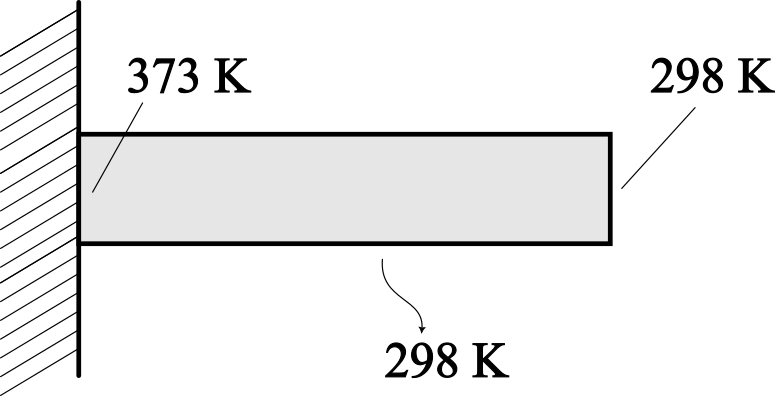
\includegraphics[width=0.5\linewidth]{figs/rod}
	\caption{Heat flow problem}
	\label{fig:rod}
\end{figure}

\section*{1D steady-state heat diffusion}
Let's first consider the steady-state formulation of the problem, where Eq. \ref{eq: heat_eq} simplifies to:
\begin{equation}\label{eq: heat_eq_ss1}
	0 = k\pdv[2]{T}{x} - h(T-T_{ext}).
\end{equation}
Isolating the spatial derivative, one gets:
\begin{equation}\label{eq: heat_eq_ss2}
	\pdv[2]{T}{x} = \frac{h}{k}(T-T_{ext}).
\end{equation}
The LHS of Eq. \ref{eq: heat_eq_ss2} can be discretized by means of a central difference scheme (CDS), as:
\begin{equation}\label{eq: heat_eq_ss3}
	\frac{T_{k-1}-2T_{k}+T_{k+1}}{\Delta x^2} =  \frac{h}{k}(T_k-T_{ext}).
\end{equation}
Defining $ \alpha =  -\frac{h \Delta x^2}{k} $, one gets:
\begin{equation}\label{eq: heat_eq_ss4}
	T_{k-1}-2T_{k}+T_{k+1} = \alpha (T_k-T_{ext}).
\end{equation}
Eq. \ref{eq: heat_eq_ss4} must be rearranged to bring the unknown $ T_k $ to the LHS:
\begin{equation}\label{eq: heat_eq_ss5}
	T_{k-1}-(2+\alpha)T_{k}+T_{k+1} = -\alpha T_{ext}.
\end{equation}
Finally, Eq. \ref{eq: heat_eq_ss5} can be assembled into a tri-diagonal linear system.

\section*{1D transient heat diffusion}

See \href{https://www.youtube.com/watch?v=CDSM5bLy8lU}{Video}

\section{2D transient heat diffusion (FDTD)}

See \href{https://sites.ualberta.ca/dept/chemeng/courses/che374/F07/notes/pdes.pdf}{Slides}

\end{document}